% \documentclass[conference, onecolumn]{IEEEtran}

\documentclass[letterpaper, 12pt]{article}

\usepackage{hyperref}

\usepackage{amsmath,amssymb,amsfonts}
\usepackage{algorithmic}
\usepackage{graphicx}
\usepackage{textcomp}
\usepackage{xcolor}
\usepackage[spanish,mexico]{babel}

\usepackage{biblatex}
\addbibresource{bibliografia.bib}

\graphicspath{{img/}}

\usepackage{float}
\usepackage{import}
\usepackage{xifthen}
\usepackage{pdfpages}
\usepackage{transparent}
\usepackage[center]{caption}
\usepackage{bm}

    \usepackage{listings}
    \lstset{ 
    	language=Matlab,                		% choose the language of the code
    %	basicstyle=10pt,       				% the size of the fonts that are used for the code
    	numbers=left,                  			% where to put the line-numbers
    	numberstyle=\footnotesize,      		% the size of the fonts that are used for the line-numbers
    	stepnumber=1,                   			% the step between two line-numbers. If it's 1 each line will be numbered
    	numbersep=5pt,                  		% how far the line-numbers are from the code
    %	backgroundcolor=\color{white},  	% choose the background color. You must add \usepackage{color}
    	showspaces=false,               		% show spaces adding particular underscores
    	showstringspaces=false,         		% underline spaces within strings
    	showtabs=false,                 			% show tabs within strings adding particular underscores
    %	frame=single,	                			% adds a frame around the code
    %	tabsize=2,                				% sets default tabsize to 2 spaces
    %	captionpos=b,                   			% sets the caption-position to bottom
    	breaklines=true,                			% sets automatic line breaking
    	breakatwhitespace=false,        		% sets if automatic breaks should only happen at whitespace
    	escapeinside={\%*}{*)}          		% if you want to add a comment within your code
    }


\begin{document}

\title{
Péndulo Simple\\
Análisis, simulación y construcción\\
}


\author{
    Enrique Benavides Téllez, Isaac Ayala Lozano,\\ 
    Sandy Natalie Campos Martínez,\\
    Luis Gerardo Almanza Granados\\
    y Yair Casas Flores
}

\date{}

\maketitle

\begin{abstract}

% El sistema del péndulo simple es uno de los sistemas más estudiados
% en teoría de control. 
% Su diseño y contrucción de baja dficultad hacen de este sistema uno de
% los más accesibles para modelar y contrastar con una implementación
% física.
% El documento presente muestra el estudio del sistema sin linearización.
% El estudio comprende la obtención de las ecuaciones de movimiento,
% la simulación del mismo en MATLAB y la comparación del modelo con
% un sistema físico.


Se presenta el desarrollo de un modelo matemático
para el péndulo simple mediante tres formulaciones de mecánica: 
mecánica Newtoniana, mecánica Lagrangiana y mecánica Hamiltoniana.
Se incluyen los resultados de los simuladores desarrollados 
en MATLAB.
Se hace una comparación de los modelos matemáticos 
con una implementación física del péndulo simple empleando el 
kit de LEGO Mindstorm.

\end{abstract}

% % \begin{IEEEkeywords}
% \end{IEEEkeywords}


El mecanismo de péndulo simple es ....

\section{Marco Teórico}

\subsection{Péndulo simple}

Para su estudio, el péndulo simple se describe como una masa 
\emph{m} concentrada en un punto \cite{sastry2013nonlinear} 
que se encuentra suspendida mediante un elemento de masa 
despreciable y de longitud \emph{l} que la conecta a un 
punto de pivoteo.
Para el trabajo presentado, las fuerzas que actúan
sobre dicha masa se restringen a la fuerza de gravedad $F_{mg}$, 
la cual induce el movimiento del cuerpo, y una
fuerza de fricción viscosa $F_f$, la cual amortigua el sistema
y lo lleva al reposo después de un tiempo dado.\\

La representación del péndulo simple puede ser observada en la
figura \ref{fig: simple pendulum}. 
La posición angular $\theta$ de la masa es medida 
respecto a la vertical del sistema.
A su vez, la figura \ref{fig: pendulum forces} presenta las fuerzas que
actúan sobre la masa.

\begin{figure}[ht]
    \centering
    \import{./img/}{pendulum_diagram.pdf_tex}
    \caption{Sistema de Péndulo simple.}
    \label{fig: simple pendulum}
\end{figure}

 \begin{figure}[ht]
    \centering
    \import{./img/}{pendulum_forces.pdf_tex}
    \caption{Diagrama de fuerzas.}
    \label{fig: pendulum forces}
\end{figure}


\subsection{Leyes de movimiento de Newton}
% https://en.wikisource.org/wiki/The_Mathematical_Principles_of_Natural_Philosophy_(1729)

Sir Isaac Newton establece en su obra \emph{Principia Mathematica} 
las tres leyes que fungen como el cimiento de la mecánica clásica 
\cite{newton1803mathematical, díaz20183d}. 
A continuación se presentan las leyes mencionadas.

\begin{enumerate}
 \item Un cuerpo mantiene su estatus quo, 
 respecto a un marco referencial inercial, salvo
 que una fuerza externa actúe sobre éste.\\
 
 La preservación del estatus quo de un cuerpo establece
 que la tasa de cambio de la velocidad $\bold{v}$ 
 del cuerpo es cero.
 
 \begin{equation}
  \sum \bold{F} = 0 \iff \dfrac{d \bold{v}}{dt} = 0
  \label{eq: 1st law of motion}
 \end{equation}

 \item La tasa de cambio de la cantidad de movimiento 
 (momentum) $\bold{p}$ de un cuerpo
 es directamente proporcional a la fuerza aplicada.
 \begin{equation}
  \bold{F} = \dfrac{d \bold{p}}{dt}
  \label{eq: 2nd law of motion}
 \end{equation}
 
 La cantidad de movimiento de un cuerpo se define como el 
 producto de la masa del cuerpo y el vector de velocidad 
 del mismo ($\bold{p} = m \bold{v}$). 
 Con esta definición es posible expresar 
 \eqref{eq: 2nd law of motion} de la siguiente manera.
 
 \begin{equation}
  \begin{split}
   \bold{F} &= \dfrac{d (m\bold{v})}{dt}\\
   &= m \bold{a}
  \end{split}
  \label{eq: conservation of linear momentum}
 \end{equation}


 \item El efecto mutuo de dos cuerpos que actúan 
 uno sobre el otro es siempre igual y en direcciones contrarias.
 \begin{equation}
  \bold{F}_{a/b} = -\bold{F}_{b/a}
  \label{eq: 3rd law of motion}
 \end{equation}

\end{enumerate}


Las leyes de Newton pueden ser aplicadas tanto a 
movimientos lineales como movimientos rotacionales.
Para el caso de la segunda ley de Newton, 
es posible extender el concepto de tasa de cambio
de la cantidad de movimiento del cuerpo 
a la tasa de cambio del momento angular $\bold{L}$
del cuerpo.
Para esta nueva expresión, el momento angular se relaciona
con el efecto que tiene el torque $\boldsymbol{\tau}$
que genera la fuerza sobre el cuerpo en cuestión.

\begin{equation}
  \sum \boldsymbol{\tau} = \dfrac{d \bold{L}}{dt}
  \label{eq: conservation of angular momentum}
\end{equation}

Considerando que el momento angular para una partícula
se define como el producto del momento de inercia 
y la velocidad angular
($\bold{L} = I \boldsymbol{\omega}$), es posible 
expresar a \eqref{eq: conservation of angular momentum}
de la siguiente manera:

\begin{equation}
 \begin{split}
  \sum \boldsymbol{\tau} &= \dfrac{d (I \boldsymbol{\omega})}{dt} \\
  &= I \boldsymbol{\alpha}
 \end{split}
 \label{eq: angular momentum and torque}
\end{equation}

\subsection{Energía}

Para una partícula solamente se consideran dos tipos de 
energía \cite{susskind2014theoretical}: la energía cinética,
relacionada con el movimiento de la partícula, y la 
energía potencial, que es una función que depende de la 
posición de la partícula en el espacio.

\begin{itemize}
 \item Energía cinética.\\
 De acuerdo a \cite{díaz20183d}, 
 la energía cinética de una partícula se expresa de 
 la siguiente manera: 
 \begin{equation}
  T = \dfrac{1}{2} m ||\bold{v}||^2
  \label{eq: kinetic energy}
 \end{equation}

 
 \item Energía potencial.\\
 La energía potencial de la partícula es una función 
 que depende de la posición de partícula, los detalles de esta 
 ecuación se presentarán en el desarrollo matemático
 del modelo.
 \begin{equation}
    V = V(x)
  \label{eq: potential energy}
 \end{equation}

\end{itemize}

\subsection{Mecánica Lagrangiana}

La mecánica Lagrangiana es un replanteamiento de la 
mecánica clásica Newtoniana, haciendo uso
de \emph{coordenadas generalizadas}
$\bold{q} = 
\begin{pmatrix}
q_1 & q_2 &\cdots & q_i
\end{pmatrix}^T
$ para describir un sistema.
Para sistemas como el péndulo simple, su uso simplifica el
desarrollo matemático del mismo.\\

Se introduce el concepto del \emph{Lagrangiano} $\mathcal{L}$,
que es una ecuación que describe la dinámica del sistema en 
función de la energía.

\begin{equation}
 \mathcal{L} = T - V(x)
 \label{eq: lagrangian}
\end{equation}

Se plantea la ecuación de Euler-Lagrange, 
que para el cálculo de variaciones permite determinar
puntos estacionarios para la ecuación funcional del sistema.
Esto permite minimizar la acción $\mathcal{A}$ del sistema.

\begin{equation}
 \dfrac{d}{dt} \dfrac{\partial \mathcal{L}}{\partial \dot{q}} - 
 \dfrac{\partial \mathcal{L}}{\partial q} = 0
 \label{eq: euler lagrange equation}
\end{equation}




%  Euler-Lagrange equation

\section{Modelo Matemático}


El péndulo simple es un sistema el cual se basa en una particula de masa $m$ sostenido de un punto fijo por medio de una barra o hilo de masa despreciable y sin extenderse mas de su distancia $l$. (Insertar figura del péndulo)\\

Para encontrar el movimiento de un péndulo se utilizaron los métodos de fuerza de Newton y el método de energías de Lagrange. Por medio del método de fuerzas de Newton, se desarrolla de la siguiente manera.
\begin{large}
\begin{gather*}
\sum F = ma = -F_{mg} - F_f \\ \bigskip
ml\ddot{\theta} = -mg\sin(\theta) - kl\dot{\theta} \\ \bigskip
\ddot{\theta} = -\dfrac{g}{l}\sin(\theta) - \dfrac{k}{m}\dot{\theta} \\
\end{gather*} 
\end{large}
\begin{flushright}
\begin{small}
m = masa del péndulo\\
l = largo del péndulo\\
k = constante fricción\\
\end{small}
\end{flushright}

El modelo en base al método de Newton se basa en conocer las fuerzas actuando, las fuerzas principales que actúan sobre el péndulo es la fuerza ocasionada por el peso de la masa ($F_{mg}$) y la fuerza de al fricción que se opone al movimiento del péndulo ($F_f$).\\

El segundo método utilizado para encontrar las ecuaciones de movimiento fue el de energías de Lagrange.
\begin{large}
\begin{equation} \label{L_equ}
\dfrac{d}{dt} \dfrac{\partial L}{\partial \dot{\theta}} - \dfrac{\partial L}{\partial\theta} = 0
\end{equation}
\end{large}
Por este método se necesitan desarrollar las ecuaciones de energía del péndulo. Y para desarrollar las ecuaciones de posición asignamos el marco de referencia del péndulo y se obtiene:\\
\begin{equation}
\left(\begin{matrix}
x\\
y
\end{matrix}\right) = 
\begin{bmatrix}
l\sen(\theta)\\
l(1 - \cos(\theta)
\end{bmatrix}
\end{equation}

\begin{flushleft}
{\large Energía Cinética}
\end{flushleft}
\begin{equation} \label{T_equ}
T = \frac{1}{2}mv^2 = \frac{1}{2}m(\dot{x}^2 + \dot{y}^2) 
\end{equation}
Derivando las ecuaciones de posición del péndulo obtenemos las ecuaciones de velocidad:
\begin{equation} \label{Vel_p}
\left(\begin{matrix}
\dot{x}\\
\dot{y}
\end{matrix}\right) = 
\begin{bmatrix}
l\dot{\theta}\cos(\theta)\\
l\dot{\theta}\sen(\theta)
\end{bmatrix}
\end{equation}
Sustituyendo la ecuación \ref{Vel_p} en \ref{T_equ} y desarrollando se obtiene:
\begin{equation}
T = \frac{1}{2}ml^2\dot{\theta}^2
\end{equation}
\begin{flushleft}
{\large Energía Potencial}
\end{flushleft}
La energía potencial se plantea multiplicando la posición en el \emph{eje y} del péndulo por la masa y gravedad. Se plantea de la siguiente manera:
\begin{equation} \label{V_equ}
V = mgl(1-\cos \theta)
\end{equation}
Con estas ecuaciones se puede definir el Lagrangiano el cual es el que va a ser diferenciado por medio de la ecuación \ref{L_equ}. El Lagrangiano se define como:

\begin{large}
\begin{align*}
L = T - V = \frac{1}{2}m(l\theta)^2 \\
= \frac{1}{2}ml^2\dot{\theta}^2 - mgl(1-\cos \theta)
\end{align*}
\end{large}

\begin{large}
\begin{equation*}
\dfrac{d}{dt} \dfrac{\partial L}{\partial \dot{\theta}} = \dfrac{d}{dt} ml^2\dot{\theta}
\end{equation*}
\end{large}
\begin{large}
\begin{equation} \label{dLv_equ}
\dfrac{d}{dt} ml^2\dot{\theta} = ml^2\ddot{\theta}
\end{equation}
\end{large}
\begin{large}
\begin{equation} \label{dLp_equ}
\dfrac{\partial L}{\partial\theta} = -gl\sin(\theta)
\end{equation}
\end{large}
Al unir la ecuación \ref{dLv_equ} menos la ecuación \ref{dLp_equ}, en base a la diferenciación del Lagrangiano (ecuación \ref{L_equ}), se obtiene la ecuación de movimiento del sistema.
\begin{large}
\begin{equation}
ml^2\ddot{\theta} + gl\sin(\theta) = 0
\end{equation}
\end{large}

\section{Simulación}

El modelo matemático obtenido se implementó en MATLAB 
para estudiar el comportamiento del sistema.
La tabla \ref{table: simulation conditions}
muestra las condiciones de simulación del programa.
El código del programa se encuentra disponible en 
GitHub\footnote{\url{https://github.com/der-coder/Cinvestav-SystemModeling-project/tree/master/codigosM}}
y se incluye como anexo.

\begin{table}[hb]
 \begin{center}
\begin{tabular}{lc}
\hline
Longitud ($l$) & 0.193 [m] \\
Masa ($m$) & 0.1232109 [kg]\\
Coeficiente de fricción ($k$) & $\{0,0.1\}$ [$N \cdot s / m$] \\
Posición angular inicial ($\theta_0$) & $0.5\pi$ [rad] \\
Velocidad angular inicial ($\dot{\theta}$) & 0 [rad/s] \\
Tiempo de simulación & 10 [s]  \\
Gravedad ($g$) & 9.81 [$m/s^2$]  \\
\hline
 \end{tabular}
 \end{center}
 \caption{Condiciones de simulación del sistema.}
\label{table: simulation conditions}
\end{table}

\subsection{Caso sin fricción}

Para el caso sin fricción, el péndulo describe 
el comportamiento armónico simple. 
Observamos que la posición angular y la velocidad angular
varían periódicamente (figura \ref{fig: time plot theta dtheta no friction}), y la amplitud máxima
del período es el mismo para cada uno de ellos.

La ausencia de fricción en el sistema no permite al sistema
encontrar un estado de reposo o estabilización. 
Esto se observa en la figura \ref{fig: phase plot theta no friction}, que
muestra el diagrama de fase del sistema.
El comportamiento del sistema describe una elipse para todos los períodos del sistema.


\begin{figure}[htb!]
 \centering 
 \import{./img/}{PosVelNF.tex}
%  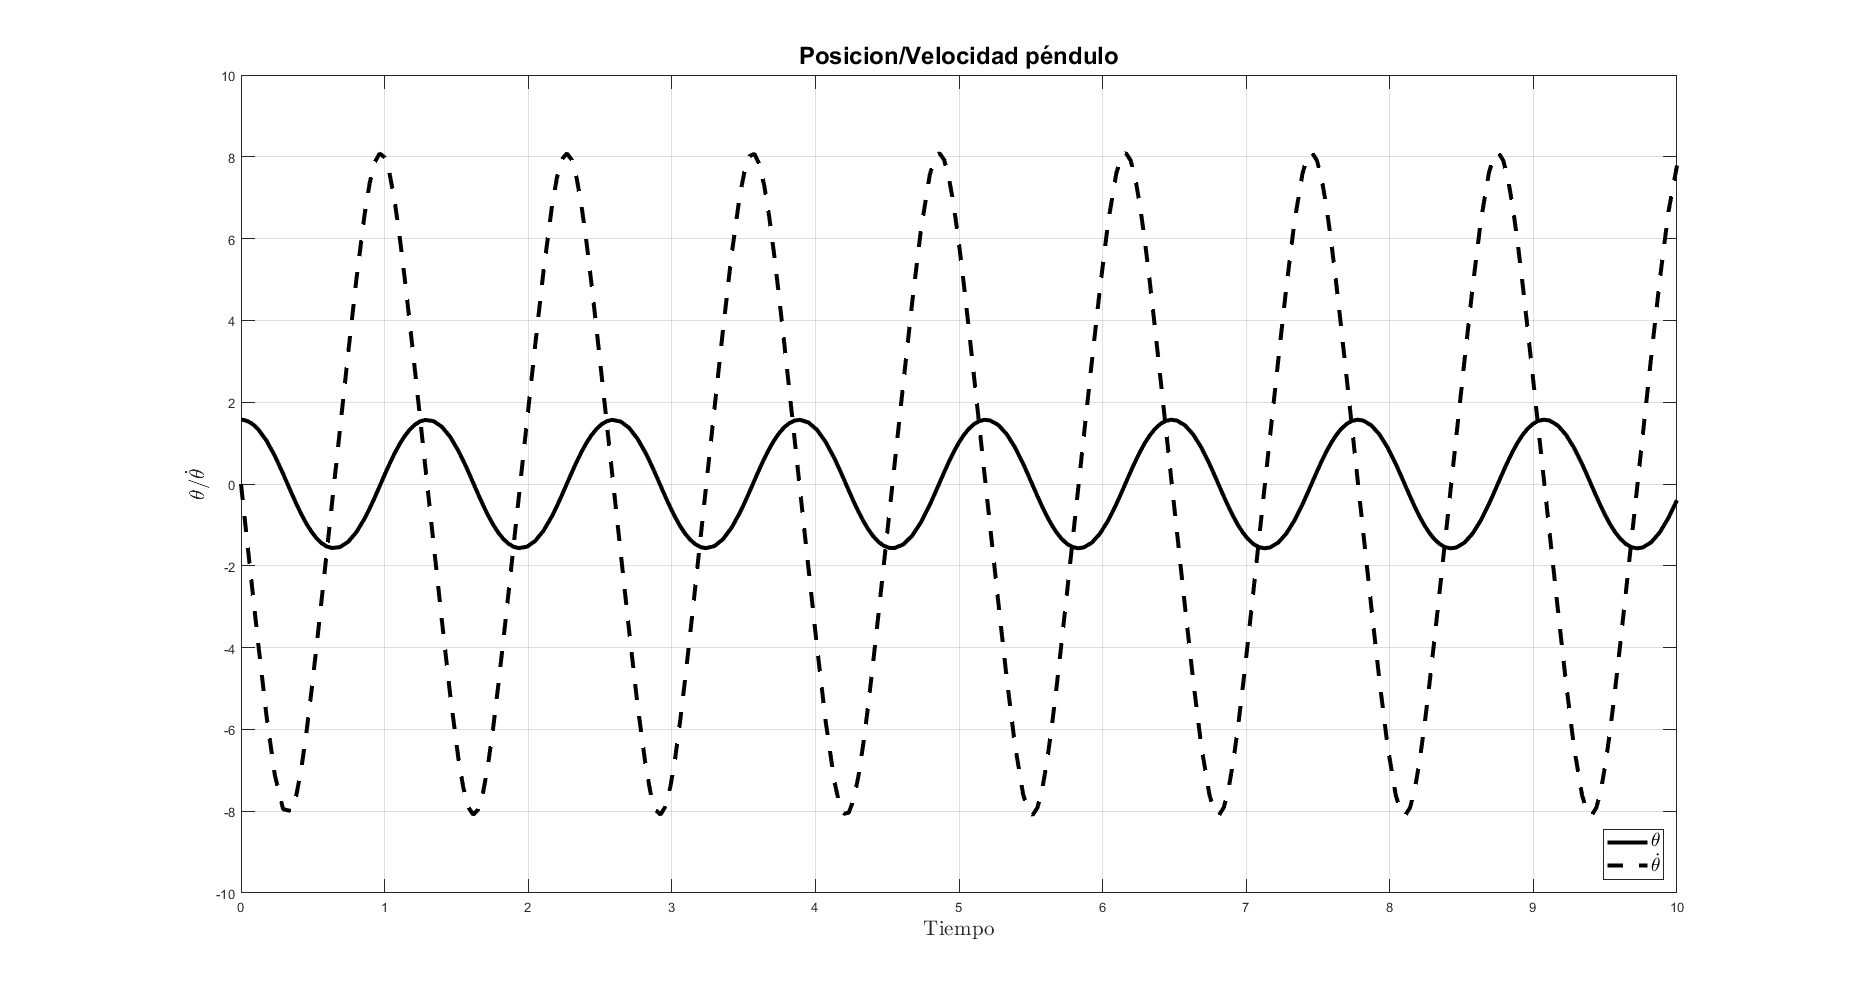
\includegraphics[scale=0.2]{PosVelNF.png}
 % fasependulox2.png: 1853x1003 px, 96dpi, 49.02x26.53 cm, bb=0 0 1390 752
 \caption{Comportamiento de $\theta(t)$ y $\dot{\theta}(t)$ en el tiempo sin fricción.}
 \label{fig: time plot theta dtheta no friction}
\end{figure}

\begin{figure}[htb!]
 \centering 
 \import{./img/}{faseNF.tex}
%  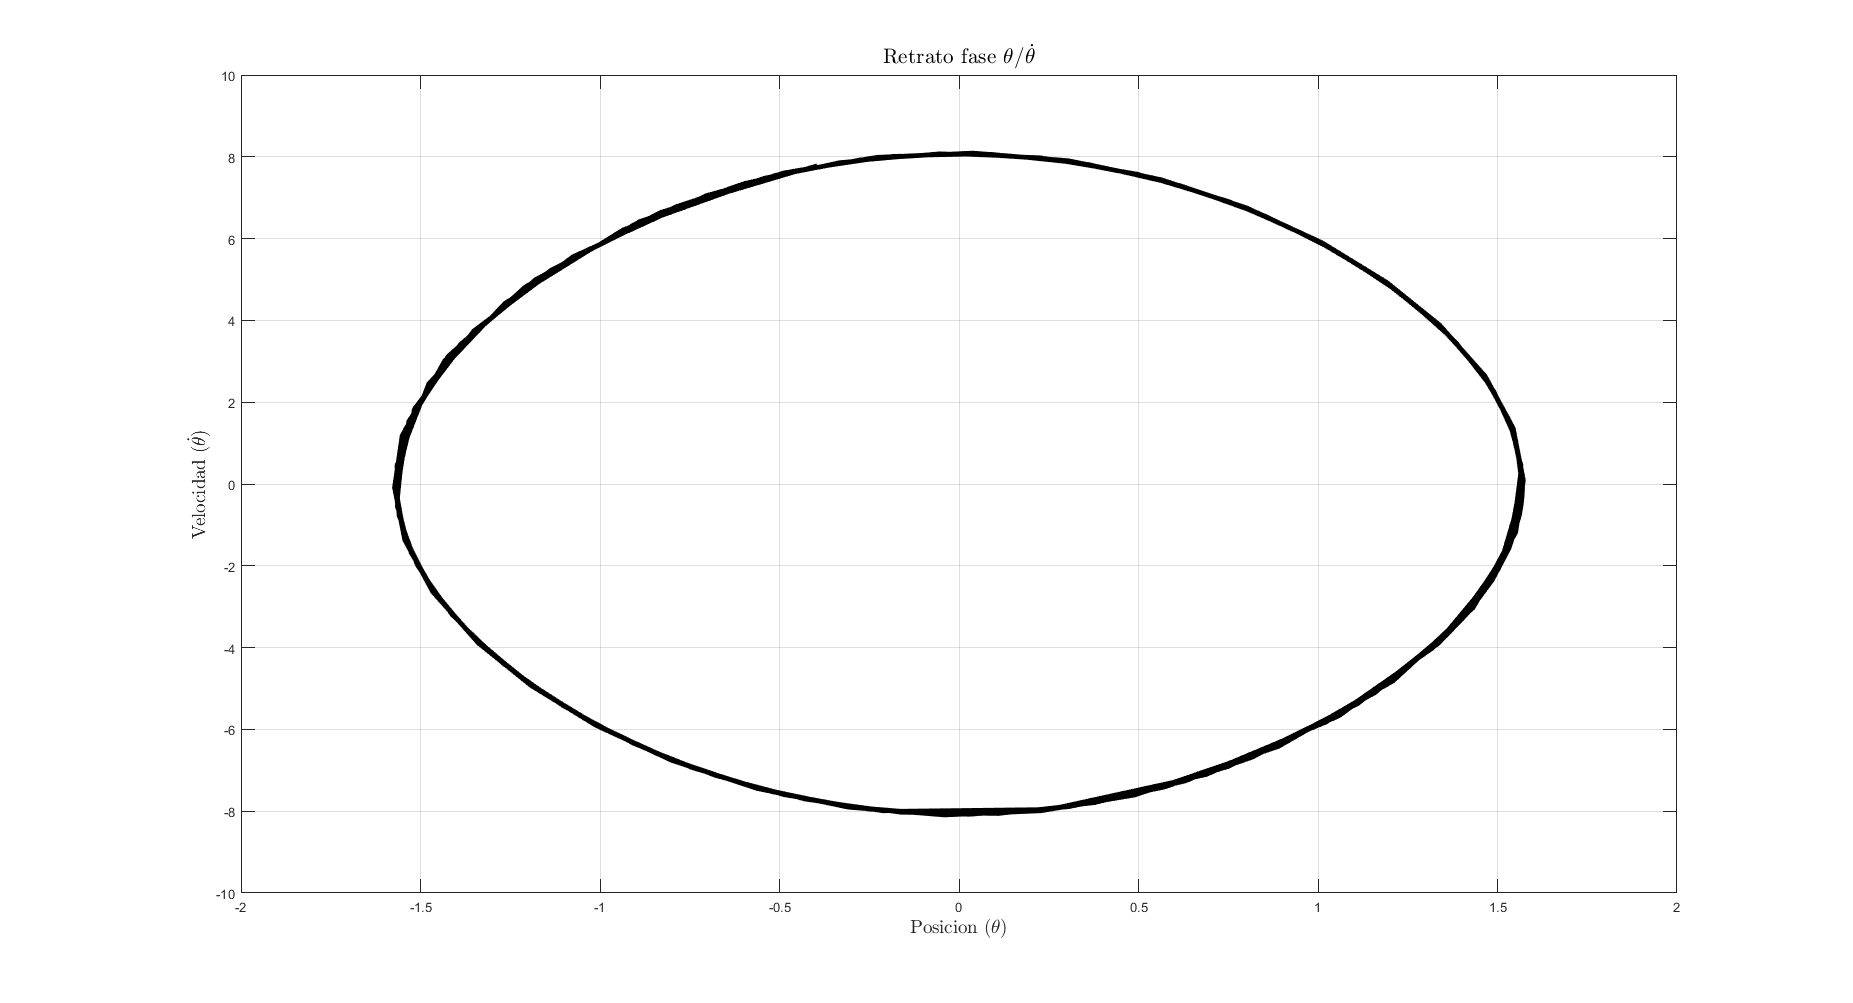
\includegraphics[scale=0.2]{faseNF.png}
 % fasependulox2.png: 1853x1003 px, 96dpi, 49.02x26.53 cm, bb=0 0 1390 752
\caption{Diagrama de fase de $\theta(t)$ y $\dot{\theta}(t)$ sin fricción.}
 \label{fig: phase plot theta no friction}
\end{figure}

\pagebreak

\subsection{Caso con fricción}
\label{simulation friction}
Se observa que el péndulo tiende a una posición de reposo debido
al efecto que la fuerza de fricción tiene sobre el sistema.
El péndulo comienza en la posición angular máxima posible 
($\theta_{max}$) y la amplitud de las crestas y valles de las 
ecuaciones disminuye para cada período de oscilación. 
Esto puede ser observado en la figura \ref{fig: time plot theta dtheta friction}.
Se observa que conforme \emph{t} se aproxima a infinito, 
la posición angular del sistema tiende al valor cero.


El diagrama de fase, mostrado en la figura 
\ref{fig: phase plot theta friction}, confirma esta tendencia.
La curva del sistema indica que tiende 
a un punto de estabilización en $\theta = 0$,
posicionando al péndulo en el eje vertical 
del marco referencial.

\begin{figure}[htb!]
 \centering 
 \import{./img/}{PosVelF.tex}
%  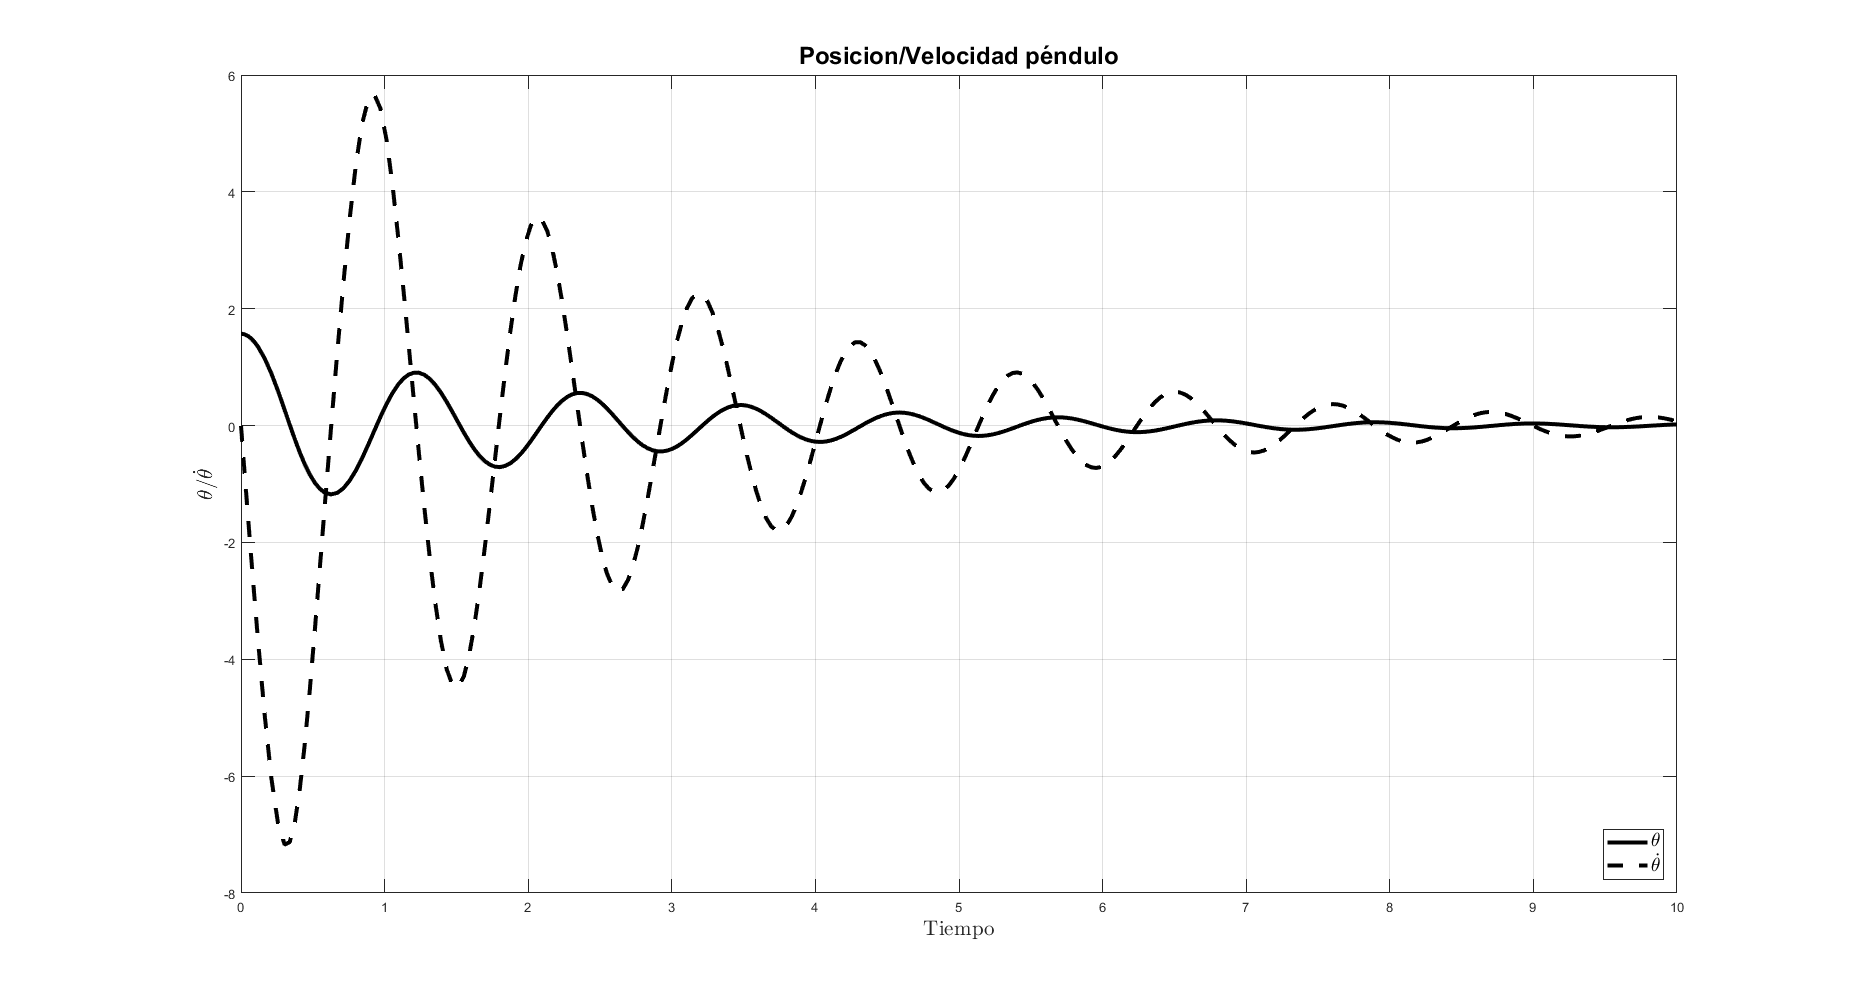
\includegraphics[scale=0.3]{PosVelF.png}
 % fasependulox2.png: 1853x1003 px, 96dpi, 49.02x26.53 cm, bb=0 0 1390 752
 \caption{Comportamiento de $\theta(t)$ y $\dot{\theta}(t)$ en el tiempo.}
 \label{fig: time plot theta dtheta friction}
\end{figure}

\begin{figure}[htb!]
 \centering 
 \import{./img/}{faseF.tex}
%  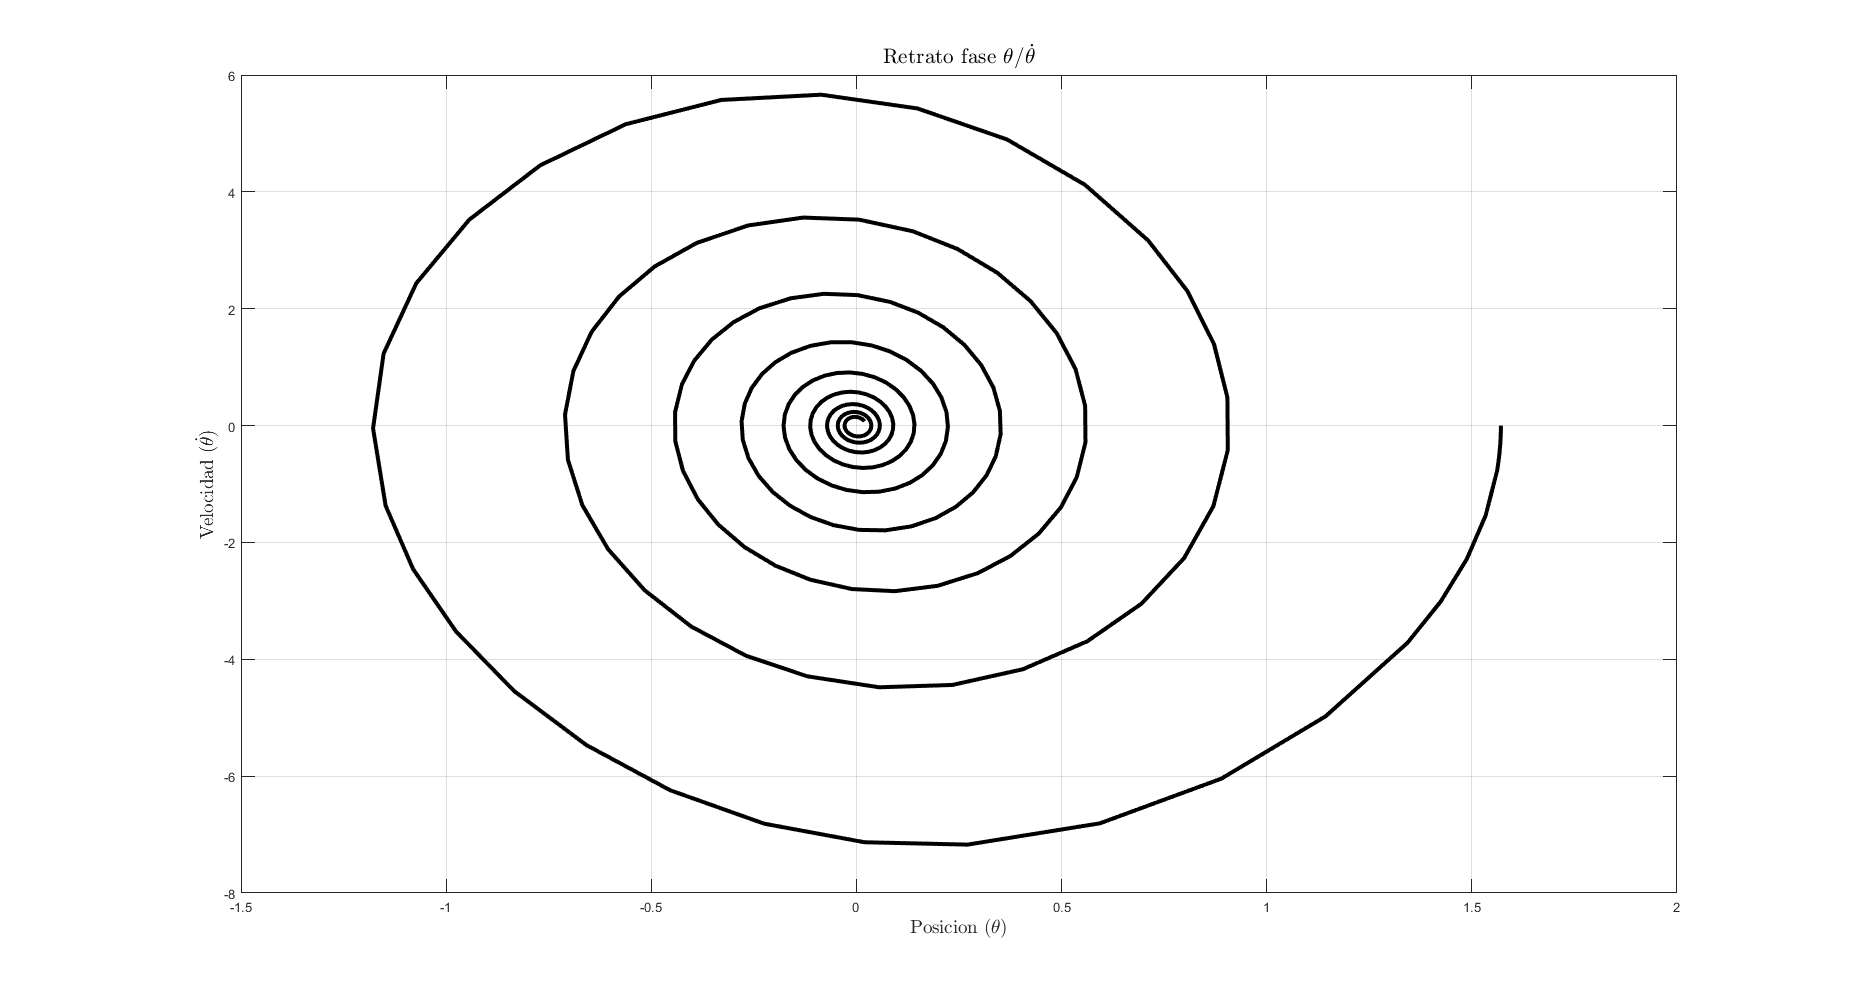
\includegraphics[scale=0.3]{faseF.png}
 % fasependulox2.png: 1853x1003 px, 96dpi, 49.02x26.53 cm, bb=0 0 1390 752
\caption{Diagrama de fase de $\theta(t)$ y $\dot{\theta}(t)$.}
 \label{fig: phase plot theta friction}
\end{figure}

\subsection{Hamiltoniano}

La formulación Hamiltoniana del péndulo fue simulada con las mismas 
condiciones que los modelos Newtonianos y Lagrangianos.
Esta simulación no contempla fricción en el sistema, produciendo
el comportamiento de un oscilador harmónico simple 
(figura \ref{fig: phase plot theta hamiltonian}).
El diagrama fase en la figura \ref{fig: phase plot theta hamiltonian}
presenta un comportamiento similar a las otras simulaciones, observando
que el momento $p_{\theta}$ es expresado como un coeficiente constante
$m l ^2$ que altera la escala de la velocidad angular $\dot \theta$.


\begin{figure}[htb!]
 \centering 
 \import{./img/}{PosVelHamilton.tex}
%  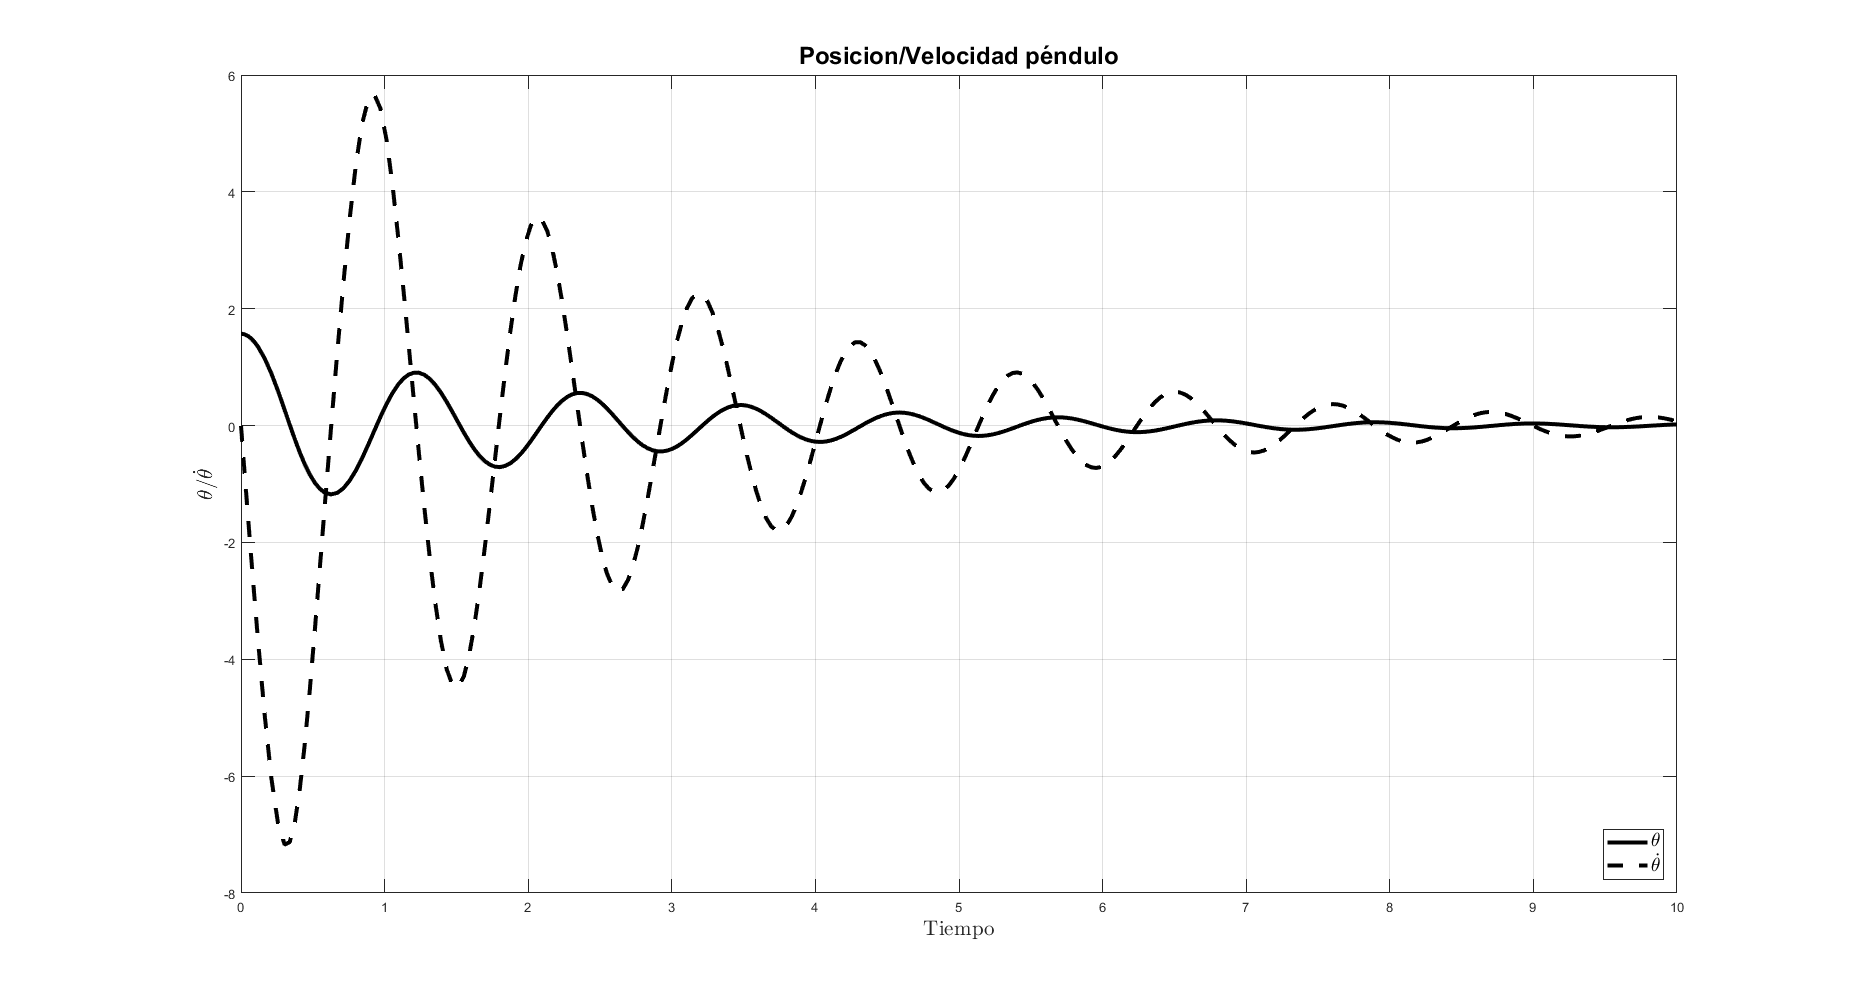
\includegraphics[scale=0.3]{PosVelF.png}
 % fasependulox2.png: 1853x1003 px, 96dpi, 49.02x26.53 cm, bb=0 0 1390 752
 \caption{Comportamiento de $\theta(t)$ y $p_{\theta}$ en el tiempo.}
 \label{fig: time plot theta ptheta hamiltonian}
\end{figure}

\begin{figure}[htb!]
 \centering 
 \import{./img/}{faseHamilton.tex}
%  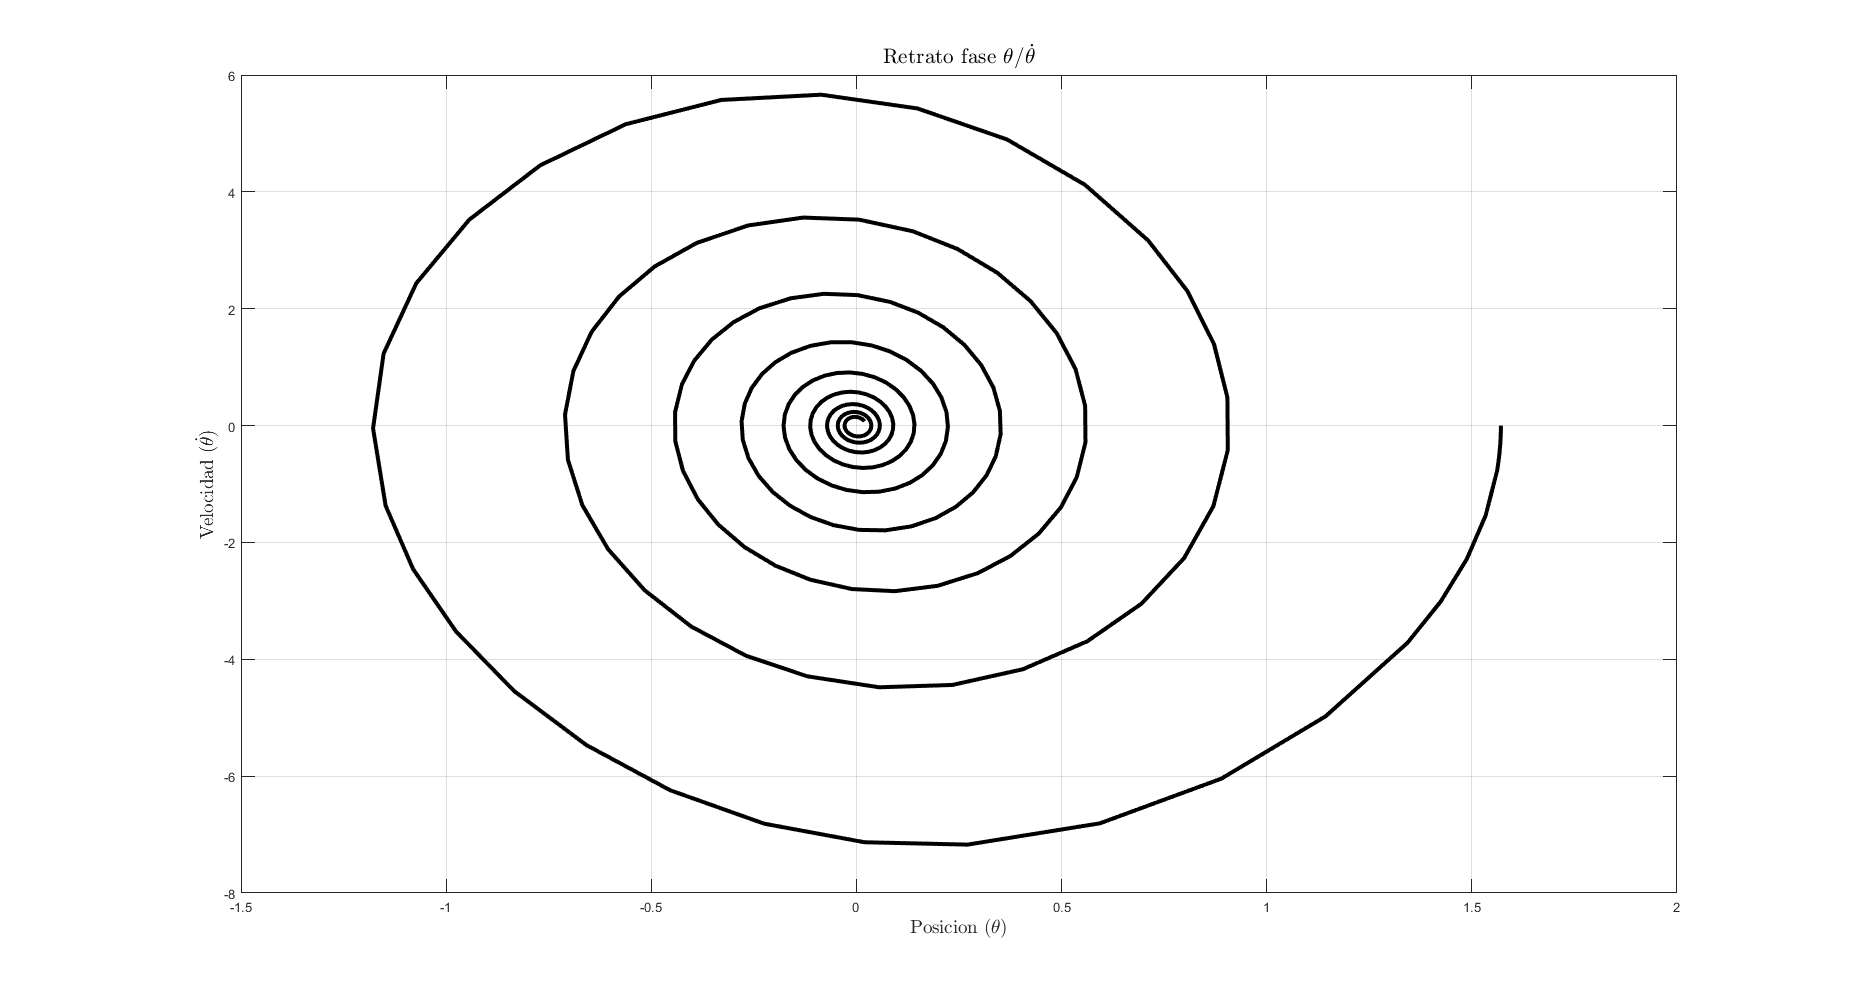
\includegraphics[scale=0.3]{faseF.png}
 % fasependulox2.png: 1853x1003 px, 96dpi, 49.02x26.53 cm, bb=0 0 1390 752
\caption{Diagrama de fase de $\theta(t)$ y $p_{\theta}$.}
 \label{fig: phase plot theta hamiltonian}
\end{figure}

\pagebreak

\section{Modelo físico}
\subsection{Prueba de concepto}

Se construyó un péndulo simple empleando 
el paquete de construcción de LEGO Mindstorms.
Este paquete posee varias características
útiles para el estudio del sistema:
\begin{itemize}
 \item Unidad de computación integrada y programable.
 \item Modularidad de sus piezas.
 \item Facilidad de ensamble.
 \item Motores de corriente directa incluyen 
 codificadores rotatorios para retroalimentación.
\end{itemize}

\subsection{Análisis de video}

Se realizó un análisis de video del péndulo construido con 
el software de \emph{Tracker}\footnote{\url{https://www.physlets.org/tracker/}}.
El video fue grabado a 30 cuadros por segundo (fps) en resolución HD.
La figura \ref{fig: tracker theta} la posición angular del 
péndulo respecto al eje vertical, medido en radianes.
El diagrama de fase (figura \ref{fig: tracker phase diagram theta dtheta})
concuerda con el comportamiento observado en el diagrama de fase de 
la simulación con fricción.


\begin{figure}[htb!]
 \centering
%  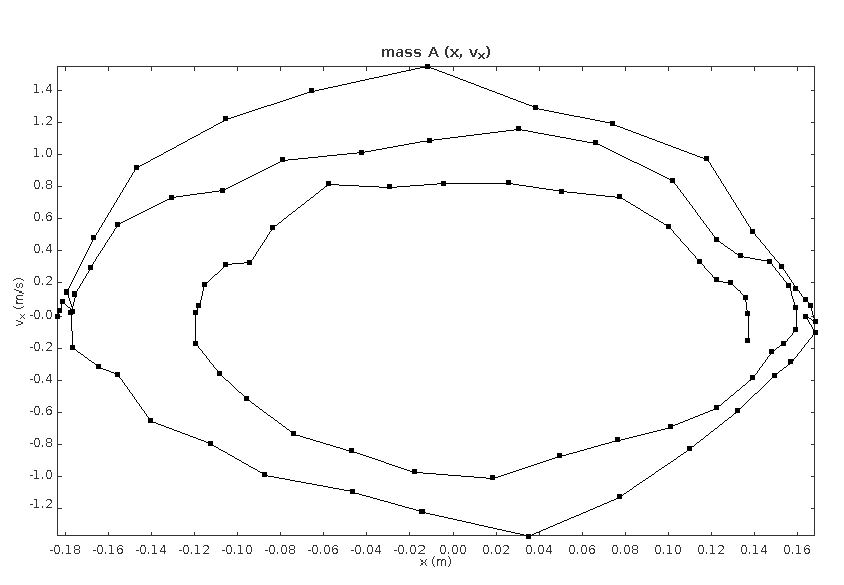
\includegraphics[scale=0.4]{./img/tracker_poc_phasediagram_x_vx.png}
\import{./img/}{pendulum_theta_tracker.pdf_tex}
 % tracker_poc_phasediagram_x_vx.png: 844x585 px, 72dpi, 29.78x20.64 cm, bb=0 0 844 585
 \caption{Diagrama de fase del modelo físico para $x$ y $\dot{x}$}
 \label{fig: tracker theta}
\end{figure}

\begin{figure}[htb!]
 \centering
%  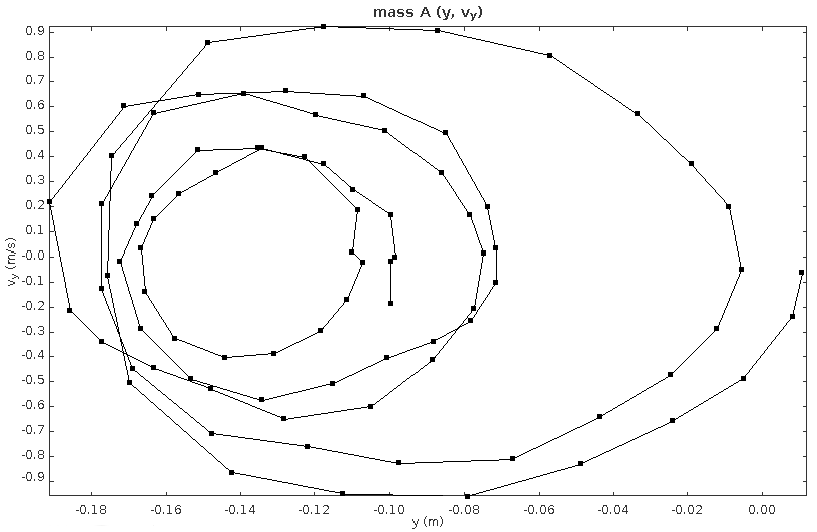
\includegraphics[scale=0.4]{./img/tracker_poc_phasediagram_y_vy.png}
\import{./img/}{pendulum_phase_tracker.pdf_tex}
 % tracker_poc_phasediagram_x_vx.png: 844x585 px, 72dpi, 29.78x20.64 cm, bb=0 0 844 585
 \caption{Diagrama de fase del modelo físico para $\theta$ y $\dot \theta$}
 \label{fig: tracker phase diagram theta dtheta}
\end{figure}


\subsection{Mediciones físicas}

Empleando los sensores incluidos en el paquete de LEGO
Mindstorms, fue posible realizar mediciones de la 
posición angular del péndulo para comparar con el
modelo matemático y el análisis de video.
La figura \ref{fig: mindstorms theta} muestra la
gráfica de mediciones de $\theta$ respecto al tiempo.
Se observa que las mediciones realizadas por el sensor
fueron afectadas por el nivel de ruido introducido 
por el mismo sensor.

\begin{figure}[htb!]
 \centering
%  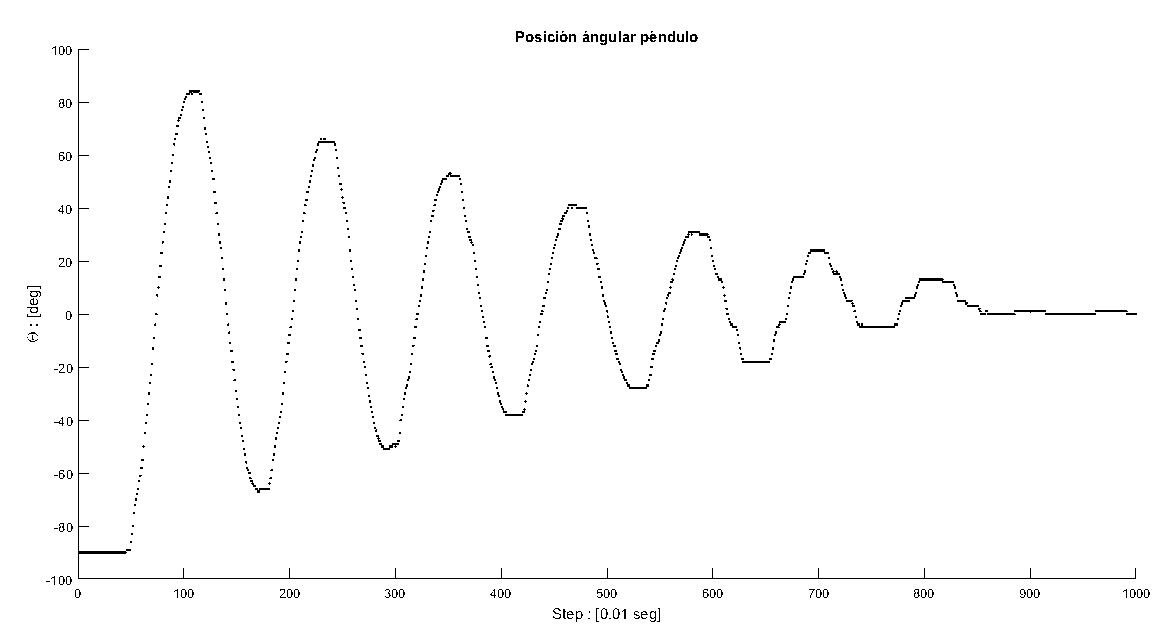
\includegraphics[scale=0.4]{../Mindstorms/Pendulin2_bw.png}
\import{./img/}{lego.tex}
 % Pendulin2_bw.png: 1157x625 px, 96dpi, 30.61x16.53 cm, bb=0 0 868 469
 \caption{Mediciones de $\theta$ para el péndulo físico con el codificador rotatorio.}
 \label{fig: mindstorms theta}
\end{figure}


\clearpage

% El mecanismo de péndulo simple es ....

\section{Conclusiones}
El proyecto concluye de manera exitosa.
La implementación de un modelo no lineal de péndulo simple y la construcción
de un modelo para validar los resultados producidos 
fue una experiencia bastante enriquecedora.
Esto debido al alcance total del proyecto: modelado,
simulación, construcción, calibración y comparación.\\

Cada etapa del proyecto requirió de habilidades diferentes, así como 
de la búsqueda de información adecuada para poder avanzar con el desarrollo.
La etapa de modelado hizo uso de las distintas formulaciones de mecánica 
que fueron presentadas durante el curso.
El desarrollo del simulador a su vez requirió de habilidades de programación
 y la capacidad de desarrollar una estrategia de trabajo que permitiera integrar
 los resultados de simulación con las áreas subsecuentes: documentación y construcción.\\

Mediante el uso de múltiples herramientas de medición fue posible calibrar el 
simulador para que el modelo virtual describa un movimiento mucho 
más cercano al comportamiento del péndulo real.
Además, la integración de nuevas herramientas de análisis permitió determinar 
propiedades del sistema que no eran posibles con los sensores disponibles.
El uso de Tracker demostró ser esencial para la obtención de los nuevos valores
del sistema debido a su capacidad de obtener detalles de la mecánica del sistema
que no fueron posibles medir con las herramientas disponibles.\\

Finalmente, el planteamiento del sistema bajo las distintas formulaciones 
de mecánica permiten obtener nuevas perspectivas sobre el modelado de sistemas.
Las formulaciones basadas en energía demuestran su poder ser adaptadas
de manera más fácil a cualquier conjunto de coordenadas.
Esta ventaja sobre la formulación de Newton resulta atractiva para modelos más complejos.
No obstante es esencial tomar en cuenta qué restricciones tienen estas formulaciones
y si es posible extenderlas para incluir los efectos de fuerzas no conservativas.



\clearpage
% \bibliographystyle{IEEEtran}
\printbibliography{}

\pagebreak

\appendix
\section{Código MATLAB}
\lstinputlisting[language=Matlab]{../codigosM/pendulin.m}

\section{Código MATLAB - Hamiltoniano}
\lstinputlisting[language=Matlab]{../codigosM/Pen_H.m}

% \pagebreak
% \lstinputlisting[language=Matlab]{../codigosM/PenduloProy.m}

\end{document}



